\begin{figure}
  \centering
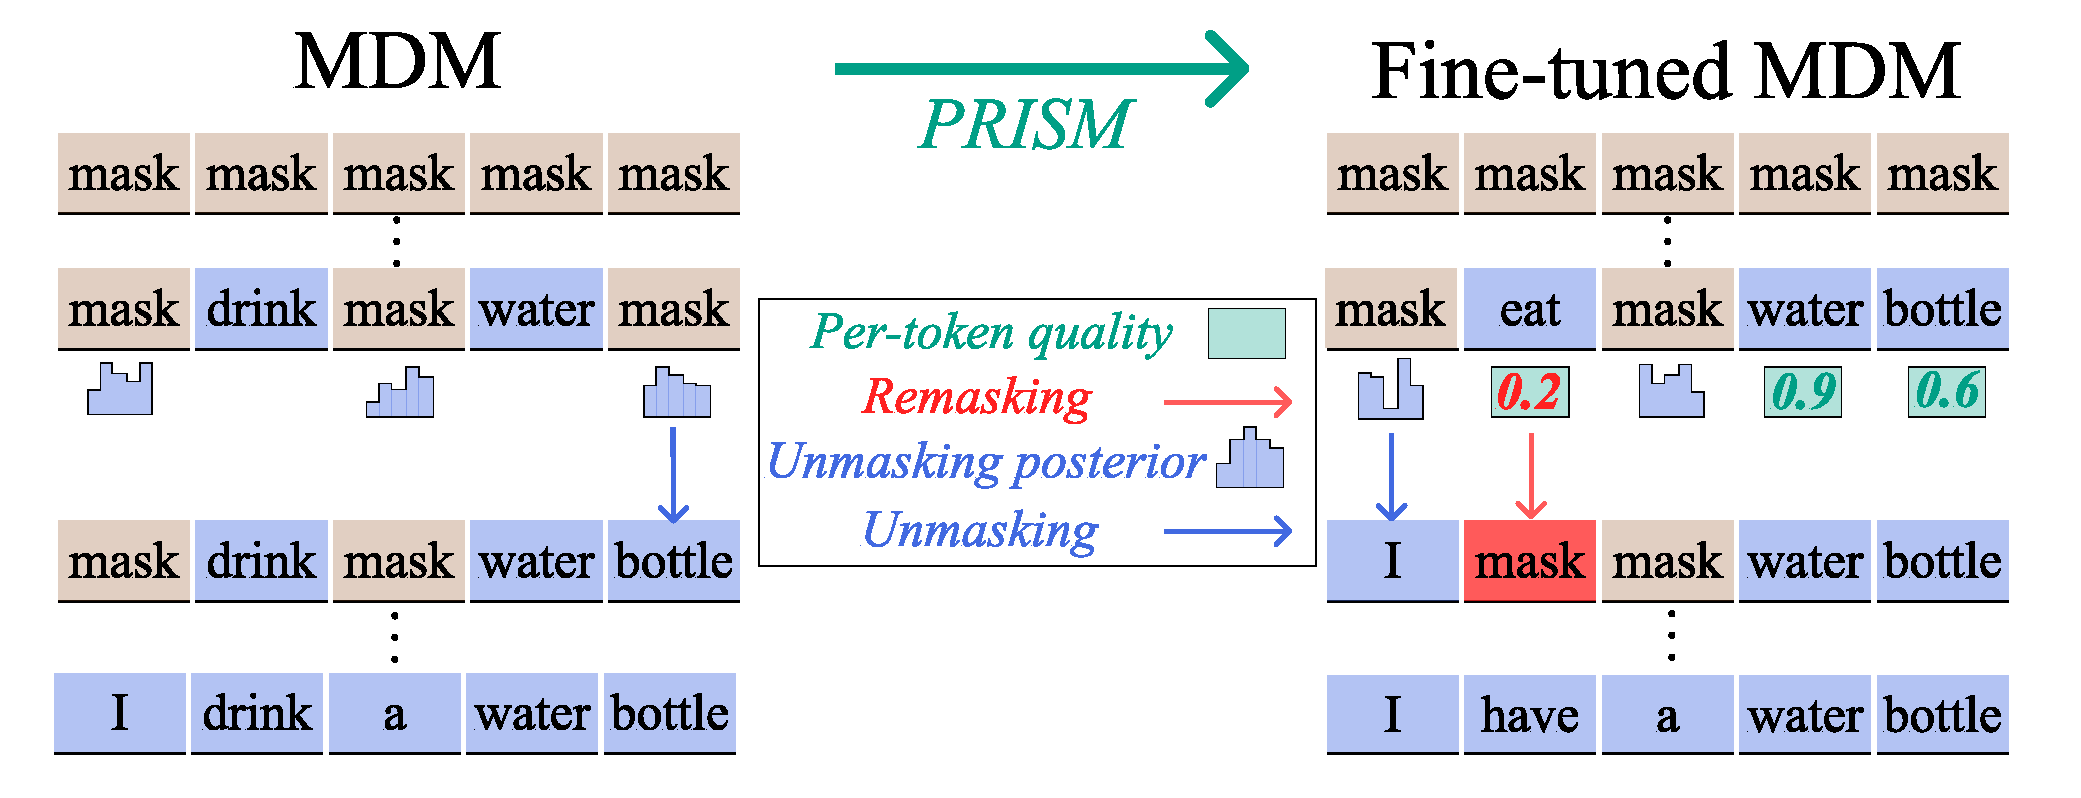
\includegraphics[width=\linewidth,trim={0 1.0cm 0 1.0cm}]{figs/PRISM_main.pdf}
  \caption{\textbf{PRISM overview}. MDMs learn an \xblue{\emph{unmasking posterior}} to unmask tokens, after which they remain fixed (\textbf{Left}). PRISM fine-tuning introduces \xxgreen{\emph{per-token quality}}, which is used to detect incorrect tokens and \xred{\emph{remask}} them. At inference, the fine-tuned MDM jointly computes \xblue{\emph{unmasking posterior}} and \xxgreen{\emph{per-token quality}}, respectively performing unmasking and remasking (\textbf{Right}).}
   \vskip -0.5\baselineskip
\end{figure} \label{fig:main}
\section{Preliminaries}
\subsection{Masked Diffusion Models} \label{sec:prelim_mdm}
\textbf{Notation.} Assume we aim to learn the distribution over sequences of length $L$ with vocabulary  $\mathcal{V}$, e.g., natural language, namely the true distribution $\rvx\sim p_{\mathrm{data}}$. $\rvx^i$ denotes the $i$-th element of a given sequence $\rvx=(\rvx^1, \dots, \rvx^L)$ and $\Delta(\mathcal{V})$ indicates the simplex of probability distributions over $\mathcal{V}$.

\textbf{MDM training.} Although MDMs can be interpreted from several viewpoints, we adopt an \emph{any-order} language model viewpoint~\citep{ou2024your,zheng2024masked}, which is essential to understanding our \PRISM framework. Roughly speaking, MDM learns the posterior marginals over clean tokens in each masked position, conditioned on a partially masked sequence. We now formalize how this objective is defined and trained. To \emph{learn} the posterior, MDM performs a \emph{masking process} using an auxiliary mask token $\mask$. For a given $\rvx\sim p_{\mathrm{data}}$, this masking process samples a partially masked sequence $\rvz\in(\mathcal{V}\cup\{\mask\})^L$ defined in two equivalent ways (see Appendix~\ref{appendix: marginal equality} for equivalence):
\begin{itemize}[leftmargin=20pt,itemsep=0pt,topsep=-0.25em] 
\item[(1)] Draw $n\sim\mathrm{Unif}\{0,\dots,L\}$ and replace the tokens at uniformly selected $n$ indices in $\rvx$ with $\mask$.
\item[(2)] Draw $t\sim\mathrm{Unif}[0,1]$ and for each $i$, replace $\rvx^i \in\mathcal{V}$ with $\mask$ with probability $t$.
\end{itemize}
To clarify, in (1), for a given $n$, we uniformly sample an index set from all size-$n$ subsets of $\{1,\dots,L\}$, and mask corresponding positions of $\rvx$. This masking process defines a random variable $\rvz$ conditioned on $\rvx$, and marginalizing it over $\rvx\sim p_{\mathrm{data}}$ \coloredhl{xblue}{induces a joint distribution over $(\rvx,\rvz)$}. 

We refer to the resulting coordinate-wise posterior conditioned on $\rvz$ as the \coloredhl{xblue}{\emph{unmasking posterior}}; $p(\rvx^i=\cdot\,|\,\rvz)$, i.e., the distribution over clean tokens at position $i$ given a partially masked sequence $\rvz$. This unmasking posterior is the core modeling component in MDM and is parameterized by a neural network $f_\theta$, which takes $\rvz$ as an input and outputs a tensor of shape $|\mathcal{V}|\times L$. Its $i$-th column, $f_\theta^i(\cdot\,|\,\rvz)\in\Delta(\mathcal{V})$, models the unmasking posterior $f_\theta^i(v\,|\,\rvz) \approx p(\rvx^i=v\,|\,\rvz)$. To train $f_\theta$, MDM minimizes the following loss:
\begin{equation} \label{eq:unmasking_loss}
    \mathcal{L}(\theta)\colon =  \mathbb{E}_{\rvx,\rvz}\left[\frac{1}{n}\sum_{i\colon \rvz^i=\mask} -\log f_\theta^i(\rvx^i \,|\,\rvz) \right],
\end{equation}
which is the cross-entropy loss summed over all masked indices. Here, the expectation is taken over the joint distribution of $(\rvx,\rvz)$ defined above. As desired, the unique minimizer $f_{\theta^\star}$ of the loss $\mathcal{L}_\theta$ satisfies $f_{\theta^\star}^i(v\,|\,\rvz)= p(\rvx^i=v\,|\, \rvz)$. This connects the MDM training loss to any-order language models such as BERT~\citep{devlin2019bert}, which model the posterior marginals at all masked positions. We note that the training loss~\eqref{eq:unmasking_loss} allows other equivalent formulations, as developed in previous MDM works~\citep{nie2025large,sahoo2024simple,shi2024simplified}.

\textbf{MDM inference.} MDM inference starts from a length-$L$ masked sequence $\rvx_1 = (\mask,\dots,\mask)$ and proceeds over a monotonically decreasing sequence of times $t_0=1>\dots>t_N = 0$. At each step $t_\ell$, given partially masked sequence $\rvx_{t_\ell}\in(\mathcal{V}\cup \{\mask\})^L$, we proceed by two steps to obtain $\rvx_{t_{\ell+1}}$:
\begin{itemize}[leftmargin=17pt,itemsep=0pt,topsep=-0.25em]
\item[(a)] Choose a subset of masked tokens $\mathcal{S}$ to \coloredhl{xblue}{unmask}, $\mathcal{S}\subseteq\{i\,|\,\rvx_{t_\ell}^i=\mask\}$.
\item[(b)] For each $i \in \mathcal{S}$, \coloredhl{xblue}{unmask} $\rvx_{t_\ell}^i$ to a clean token sampled from $f_\theta^i(\cdot\,|\, \rvx_{t_\ell})\in\Delta(\mathcal{V})$.
\end{itemize}
Notably, step (a)—the choice of $\mathcal{S}$—is highly flexible and central to MDM’s gains on downstream tasks; $\mathcal{S}$ may be chosen arbitrarily. Two predominant strategies are independently including each masked index $\rvx_{t_\ell}^i=\mask$ with a fixed probability~\citep{sahoo2024simple, shi2024simplified} or adaptively selecting indices, e.g., the most confident tokens or the leftmost tokens~\citep{chang2022maskgit,zheng2023reparameterized,kim2025train,nie2025large}.

\subsection{Self-correction for MDM via per-token quality} \label{sec:prior_work_main}

An ideal generative model would detect low-quality tokens at inference time and correct them when appropriate. Prior work has explored self-correction in LLMs, including \cite{kumar2024training,gou2023critic}, and, recently, in MDMs. Despite varying instantiations, these methods for MDM can be organized into a common two-step procedure. At each inference step, given $\rvx_{t_\ell}$:
\begin{itemize}[leftmargin=17pt, noitemsep, parsep=3pt, topsep=0pt]
    \item[(a)] Compute a per-token ``quality score'' for each $\rvx_{t_\ell}^i\ne \mask$ and, according to it, select a subset of clean tokens $\mathcal{T}$ to \coloredhl{xxgreen}{remask}.
    \item[(b)] For each $i\in\mathcal{T}$, \coloredhl{xxgreen}{remask} $\rvx_{t_\ell}^i$ and either replace it with a new clean or leave it masked.
\end{itemize}
At step (a), the set $\mathcal{T}$ is typically chosen with the lowest per-token quality, optionally with stochasticity. At step (b), the remasked $\rvx_{t_\ell}^i$ can be immediately resampled (using the pretrained model or an auxiliary module) or kept to engage further for future unmasking/remasking steps. Combined with the standard MDM unmasking step (Section~\ref{sec:prelim_mdm}), inference alternates between unmasking and (re)masking; these may be interleaved or staged, depending on the method.

\textbf{Challenge.} 
The key challenges are twofold: formulating a \coloredhl{xxgreen}{\textbf{principled definition of per-token quality}} and \coloredhl{xxgreen}{\textbf{constructing a model}} that estimates it. These can be formalized as follows: A per-token quality is a function $g_\star$ that takes any partially masked sequence $\rvy$ and returns position-wise scalars for non-masked positions $\rvy^i\ne\mask$:
\begin{equation*}
    g_\star\colon (\mathcal{V}\cup\{\mask\})^L \to [0,1]^L,\quad \xxgreen{g^i_\star(\rvy) \approx (\text{Per-token quality})}=(\text{``how likely'' $\rvy^i$ is given $\rvy$}).
\end{equation*}
The phrase ``how likely'' is a modeling choice; whatever the choice, it should align with the intended notion of per-token quality (our \PRISM instantiation is given in Section~\ref{sec:prism}). The goal is a computationally efficient algorithm for modeling $g_\star$ that, in the limit, provably learns the chosen definition of per-token quality. As we argue next, prior work typically lacks either a precise, testable target of per-token quality or entirely changes the MDM design itself, limiting its applicability. We therefore organize the prior work along whether it specifies a precise target for per-token quality on the state during inference $\rvx_{t_j}$ and how disruptive it is to the MDM design. 

\begin{itemize}[leftmargin=10pt, noitemsep, parsep=3pt, topsep=0pt]
    \item Training-free approaches: DFM~\citep{gat2024discrete}, ReMDM~\citep{wang2025remasking}, P2-Self~\citep{peng2025pathplanningmaskeddiffusion} are drop-in and can be applied to any pretrained MDM, however they lack a precise target: scores are random (DFM, ReMDM), evaluated on a different input than $\rvx_{t_\ell}$ (ReMDM-conf), or inferred from logits that were not trained to present the token quality (P2-Self).
    \item Methods that require rehauling MDM design:  GIDD~\citep{von2025generalized}, Informed Corrector~\citep{zhao2024informed}, indeed articulate a valid target for self-correction but achieve it by changing the pretraining design or architecture, requiring full retraining. 
    \item Proxy-$\hat{\rvx}$ approaches: Token Critic~\citep{gou2023critic} and P2-Train~\citep{peng2025pathplanningmaskeddiffusion} train an external scorer to approximate the marginal likelihoods of a sampled clean sequence $\hat{\rvx}$. For a given $\rvx_{t_\ell}$, it first samples a reconstructed clean sequence $\hat{\rvx}$ via $f_\theta$ in a single step, then calculates the quality score via the trained module. Since the pretrained MDM has learned the \emph{per-token} unmasking posterior, not the \emph{joint posterior} across positions, $\hat{\rvx}$ can deviate a lot from a valid sample from the posterior. This method also requires an extra forward pass for scoring.
\end{itemize}
We provide a comprehensive explanation of the prior work and their notions of per-token quality in Appendix~\ref{appendix:prior_work}. \emph{In short}, prior work either lacks a precise target of per-token quality or alters the design of the MDM itself. \emph{In contrast}, PRISM assigns an explicit per-token target to a given sequence $\rvx_{t_\ell}$ and estimates it in a single forward pass by fine-tuning the pretrained MDM, while still preserving the MDM’s ability to compute per-token posteriors. 